\documentclass[]{article}
\usepackage{graphicx}
\usepackage{xcolor}

\parindent=0pt
\usepackage[margin=0.5in]{geometry}
\usepackage{url}
\usepackage{hyperref}
\usepackage{graphicx}

\begin{document}
\pagestyle{empty}
{\large\textbf{Research Notes}}
\begin{itemize}
    \item[*] Created on Mon 04 Jan 2016 11:23:25 AM EST
    \item[*] Modified on \today
    \item[*] Author info: Boyou Zhou\\
             8 St Mary's St, PHO 340, Boston, MA 02215\\
             Email: bobzhou@bu.edu, Phone: 617-678-8480\\
\end{itemize}

\rule[-0.1cm]{7.5in}{0.01cm}\\
\noindent \textbf{Mon 04 Jan 2016 11:14:43 AM EST}
\textit{Beginner's tutorial of AXI slave logic design}

This documents gives a brief instruction of how to design an AXI slave logic on Zedboard.
 Zedboard provides two ARM cores and programmable logic.
 From here, ps stands for GPP, ARM in this case, pl for programmable logic.\ 

Ps and Pl are connected with AXI ports. In this design, our logic talks to the
ps with AXI ports.\ ps looks at the logic as memory blocks. More strictly, the
ps visit the logic registers as memory units. On the ps side, I used a full
linux, Linaro Linux as the os for ps. The programs are run on the ps interfacing
the memory units through AXI ports, $/dev/mem$

Here are the tutorials to the design.
\indent		\begin{itemize}
			\item \textit{Start Linux}
			\url{http://fpga.org/2013/05/24/yet-another-guide-to-running-linaro-ubuntu-desktop-on-xilinx-zynq-on-the-zedboard/}
			\item \textit{AXI Slave Logic}
			\url{http://www.fpgadeveloper.com/2014/08/creating-a-custom-ip-block-in-vivado.html}
			\item \textit{Visit Memory Block}
			\url{http://fpga.org/2013/05/28/how-to-design-and-access-a-memory-mapped-device-part-one/}
        \end{itemize}

The device tree design, we do not include adv7511.dtsi in zynq-zed-adv7511.dtsi

\noindent \textbf{Thu 07 Jan 2016 12:38:46 PM EST}
\textit{Papers related to security}
\begin{itemize}
	\item side channel detection \cite{longo2015soc} 
	\item encoding methods \cite{chakraborti2015trivia} 
	\item radio security breach \cite{genkin2015stealing}
	\item PUF \cite{aysu2015end} \cite{maes2015secure} \cite{herder2014physical} \cite{devadas2010secure}
	\item SAT \cite{saha2015improved}
	\item TRNG \cite{haddad2015physical}\cite{suh2007physical}\cite{herder2014trapdoor}
	\item new tech \cite{suh2003efficient}
	
\rule[-0.1cm]{7.5in}{0.01cm}\\
\\
	\item coprocessor \cite{roy2015lightweight} 
	\item break RSA on Intel chip \cite{bhattacharya2015watches}
	\item accelerating homomorphic encryption \cite{doroz2015accelerating}
	\item memory verification and encryption, verification ensures the
adversary changes in the machine states. Encryption protects the off-chip
memory\cite{suh2003efficient}

\end{itemize}

some explanation
\begin{itemize}
	\item \cite{herder2014trapdoor}TRNG: safely extract the keys from biometric source
\end{itemize}

\rule[-0.1cm]{7.5in}{0.01cm}\\
\noindent \textbf{Mon 01 Feb 2016 09:55:39 AM EST}
\textit{Architecture people working on security}

\begin{itemize}
	\item Srini Devdas (MIT) \url{https://scholar.google.com/citations?user=-yrzguMAAAAJ&hl=en}
	\item Edward Suh (Cornell) \url{https://scholar.google.com/citations?user=neO3vFYAAAAJ&hl=en&oi=ao}~\cite{chen2015execution}
	\item Mohit Tiwari (U T Austin)
	\item Simha Sethumadhavan (Columbia)
	\item Tim Sherwood (UCSB)
	\item Dawn Song (U C Berkeley)
\end{itemize}

In the homomorphic computation, somewhat homomorphic function evaluation needs to be reviewed.\textbf{SHF}
\begin{itemize}
	\item \cite{chen2015execution} gives the 
\end{itemize}

\rule[-0.1cm]{7.5in}{0.01cm}\\
\noindent \textbf{Mon 22 Feb 2016 01:59:29 PM EST}
\textit{papers on architecture security}
\begin{itemize}
	\item \cite{wang2014timing} RSA attacks: each RSA decoding will result in
memory access. Thus the number of access in memory is the hamming distance of
RSA keys.
	\item \cite{ismail2015improving} 
	\item \cite{ancajas2014fort} thread model: HTs attacks one of the cores and
propagate information to other cores.  
        \begin{itemize}
            \item data scrambling
            \item dynamic packet certificate
            \item node obfuscation
        \end{itemize}
    \item \cite{liu2015ghostrider} 
        \begin{itemize}
            \item split the memory into three types, normal memory, encrypted memory and oblivious memory
            \item use software-directed scratchpad instead of implicit cache access
            \item deterministic processor pipeline against timing attacks
        \end{itemize}
\end{itemize}

\rule[-0.1cm]{7.5in}{0.01cm}\\
\noindent \textbf{Mon 22 Feb 2016 01:59:29 PM EST}
\textit{papers on architecture security}
\begin{itemize}
    \item \cite{diguet2007noc} Threat models:
        \begin{itemize}
            \item a write access in the secure area to modify the system behavior
            \item covert attacks
                \begin{itemize}
                    \item extraction of information
                        \begin{itemize}
                            \item RSA fault injection\cite{pellegrini2010fault} 
                            \item AES attack\cite{moradi2006generalized}
                            \item DPA \cite{kocher2011introduction}
                        \end{itemize}
                    \item communication between different applications \cite{wang2012efficient}
                \end{itemize}
            \item denial of service:
                \begin{itemize}
                    \item replay: wastes of bandwidth
                    \item incorrect path: introduce erroneous paths
                    \item deadlock: the use of packets with paths that intentionally create deadlocks
                    \item livelock: introduce packets that can never reach the end so that they stay turning in the network
                \end{itemize}
        \end{itemize}
\end{itemize}

\rule[-0.1cm]{7.5in}{0.01cm}\\
\noindent \textbf{Tue 08 Mar 2016 02:28:51 PM EST}
\begin{itemize}
    \item SNI - \textit{Secure Network Interface} 
        \begin{itemize} 
            \item DoS
            \item Unauthorized Read Access(Information Extraction) and unauthorized write access (Hijacking){\color{red}more literature review}
        \end{itemize}        
    \item bus-based control~\cite{diguet2007noc}
        \begin{itemize}
            \item overflow checking
            \item path based identification
            \item local access checking
            \item statistics
        \end{itemize}
    \item secure memory access \cite{goossens2008hardwired} extending \cite{fiorin2007data}
        \begin{itemize}
            \item design of Data Protection Units (DPUs) managed by Network Security Manager(NSM)
            \item memory security \cite{gebotys2003security}
            \item anti-side channel \cite{evain2005noc}
        \end{itemize} 
\end{itemize}

Memory Related Stuff
\begin{itemize}
    \item \cite{fiorin2007data} designed a module in memory call Data
Protection Unit. It protects requested accesses to the memory blocks through a
lookup of the access rights.
    \item \cite{gebotys2003security} prevents attacks which can obtain data
from communication network. Since keys are often updated from time to time. Noc
needs to secure the key exchanges on the network.
\end{itemize}

\begin{itemize}
	\item \cite{kocher2011introduction} introduction to differential power analysis
	\item \cite{pellegrini2010fault} RSA attack, retrieve the private key with fault based  
\end{itemize}


\rule[-0.1cm]{7.5in}{0.01cm}\\
\noindent \textbf{CSET}
\begin{itemize}
	\item metric security evaluation
	\begin{itemize}
		\item \textit{A Metric for the Evaluation and Comparison of Keylogger
		Performance}The paper provide a framework to assess the performance of
		mobile device keylogger.  The metric can measure the effectiveness of
		the software keyboard typing.
		\item \textit{DACSA:A Decoupled Architecture for Cloud Seucrity
		Analysis} The paper proposes an out-of-VM cloud analysis architecture.
		The framework measure the VM execution from the supervisor side for
		evaluating the security. The evaluation is the Ops/Sec on CPU and memory
		for different VMs.
		\item \textit{Effective Entropy:Security-Centric Metric for Memory
		Randomization Techniques} Effective entropy is a metric of indicating
		adversary workload and comparison between different kinds of
		randomization.
	\end{itemize}
	\item testing related papers 
	\begin{itemize}
		\item \textit{Safe and Automated Live Malware Experimentation on Public
		Testbenches} The paper is about testing methods for detections of
		malware during communication. They propose containment policies for
		testing malware by copy the observations and data gathered in malware
		analysis and put them locally for studying. It also includes emulation
		of testing environments.
		\item \textit{TESTREX: a Testbed for Repeatable Exploits} This paper
		designed a new testbed for packing and running applications with their
		environments, injecting exploits and monitoring their success. TESTREX
		combines the applications and their environments together for testing.
	\end{itemize}
\end{itemize}

\rule[-0.1cm]{7.5in}{0.01cm}\\
\noindent \textbf{WESS}
\begin{itemize}	
	\item \textit{A Novel Attack on a FPGA based True Random Number Generator}
	HT designed in the TRNG of FPGA to make the random number incident
	triggering rate rise from 0.5 to 0.75.
	\item \textit{CHEF:A Configurable Hardware Trojan Evaluation Framework}
\end{itemize}

\begin{figure}
	\centering
	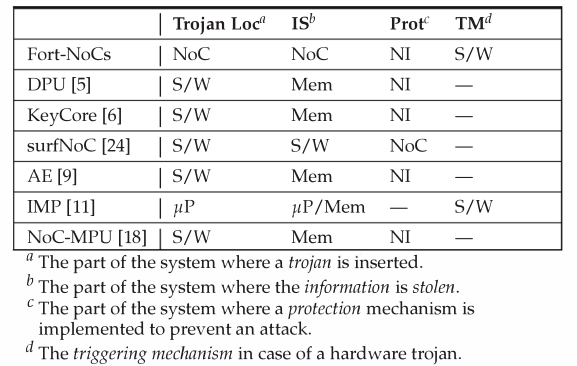
\includegraphics[width=4in]{img/defense-comparison.png}
	\caption{defense comparison}
\end{figure}

From~\cite{ancajas2014fort,js2015runtime}
\begin{itemize} 
	\item SNI/SCM	~\cite{diguet2007noc}
		Secure NIs and Secure Configuration Manager(SCM): SNI act as a filter for
	the network and handle attack symptoms that may be caused by dos attacts and
	unauthorized r/w access. SNI verifys the packet sender The SCM configures
	system and SNI.
	\item DPU		~\cite{fiorin2008secure}
		Data Protection Units, implemented within Network Interfaces, can check and
	limit the access rights (none, read, write, or both) of processors accessing
	data and instructions in a shared memory. The DPU can distinguish between
	operating roles (supervisor/user and secure/nonsecure) ofthe processing
	elements. DPU is to seperate sensitive and non-sensetive data.
	\item KeyCore	~\cite{gebotys2003framework}
		At the network level, each IP core has a security wrapper and a
	key-keeper core is included in the NoC protecting encrypted private and public
	keys. This work is to prevent untrusted software on or off onthe Noc to
	gain access to the keys.
	\item surfNoC	~\cite{wassel2013surfnoc}
		For security and many other reasons, time multiplexing is widely used
	in NoCs. It is possible to isolate data without time multiplexing in order to
	boost performance.
	\item AE		~\cite{kapoor2013security}
		Authenticated Encryption security framework for NoC based system. The
	communications between IP secure cores use permenant keys, while the
	communications between unsecure and secure cores use session keys.
	\item IMP		~\cite{king2008designing}
		Illinois Malicious Processors(IMPs) Design of malicious circuit design
		to faciliate attacks. The paper consider two machenisms. A memory access
        mechanism that provides unchecked memory accesses and allows an attacker
        to bypass the protection of the memory management unit. A shadow mode
        mechanism that allos the attackers to execute an invisible malicious
        firmware.
	\item NoC-MPU	~\cite{porquet2011noc}
        MPU is a memory protection unit allowing to support the secure and
        flexible co-hosting of multiple native software stacks running in
        multiple protection domains.
\end{itemize}

% Here, we can assume that routers have been compromised and inserted some
% trojan, but we need to list what kind of HTs has been inserted. I assume that
% there should be HTs can capture the packets on the network and extract
% information from them. We target threats of information extraction.
We assume that the data communication channel has been compromised.
\begin{itemize}
	\item \cite{lim2005extracting} illegal r/w leads to key information leakage
	\item \cite{fiorin2008implementation,sepulveda2012hybrid,kim2009trojan} use verifications/look-up tables to prevent malicious request
	\item \cite{sajeesh2011authenticated} encryption authorization?
	\item \cite{fiorin2009mpsocs} internal probing
	\item \cite{diguet2007noc} exchange secrets through covert channels
\end{itemize}

\rule[-0.1cm]{7.5in}{0.01cm}\\
\noindent \textbf{Mon 04 Apr 2016 12:05:44 PM EDT}
\begin{table}[!t]
	\centering
	\begin{tabular}{c l l}
		Paper & Threat & Defense Mechanism\\
	\hline
	% NOC-centric security of reconfigurable SoC
	~\cite{diguet2007noc} 	& Hijacking, extraction of information and DoS  	& SNI and SNM design\\
	sw					  	& attacks,											& SNM is in charge of SNI configuration. It monitors network.\\
						  	& excluding side channel or fault injection 		& SNI has defense against Dos,information extraction and\\
						  	& The threat models are based monitoring  			& hijacking. The system can be reconfigured once\\
						  	& reconfiguration									& an attack is detected.\\
							&													& It also proposed a routing technique: the choice of\\
							&													& output port is given by the turn number in counter\\
							& 													& clock-clockwise from considered input port. In this way,\\
							& 													& the receiver knows who the sender is.\\
	\hline
	% Secure Memory Accesses on NOCs
	\cite{fiorin2008secure} & Buffer overflow or other illegal method accessing & Network Security Manager acts as supervisor of the network.\\
	sw						& memeory, and snooping attacks 					& Data Protection Unit acts as the firewall of the memory.\\
							& 													& The system prevents snooping attacks by verification\\
							& 													& from the source processor. Snooping attacks can be done\\
							& 													& by modifing the processor identifier.\\
	\hline
	% SurfNoC: a new latency and provably non-interfering approach to secure networks-on-chip
	\cite{wassel2013surfnoc}& Alternative of time-multiplexing to protect Nocs  & The paper proposes the idea of alternatively using the link\\
	isolation				&													& so that in each cycle, the packet can be forwarded. This \\
							& 													& increases the throughput of the entire network. The author\\
							& 													& claims that once the packet has been passed on the network,\\
							& 													& it does not need to wait due to time multiplexing.\\
	\hline
	% A security framework for noc using authenticated encryption and session key
	\cite{kapoor2013security}& Extraction of important information from IP 		& \textit{related work contains attacks from one core to another}\\
	sw						& cores												& A seperate module distributes temporary session key  \\
							&      												& for secure and non-secured IP cores communications.  \\
							&      												& The non-secure cores use temperory session keys to  \\
							&      												& communicate with secure cores so that they can not re-use  \\
							&													& the keys to send malicious packets.\\
	\hline
	% Fort-Nocs: Mitigating the Threat of a compromised Noc
	~\cite{ancajas2014fort} & HT in router forward message to accomplice thread & Data encryption with XOR cipher encryption \\
	sw and hw				&													& packet certificate, suppose firmware of cores have not been \\
							& 													& tampered\\
							&													& node obfuscation, previously done by noise injection\\
							& 													& here, done by migration of applicaitons as a routine\\
	\hline
	% Fault-based attack of RSA authentication
	~\cite{pellegrini2010fault} & fault injection to break RSA					&\\
	hw						&													&\\
	\hline
	% Exploiting Error Control Approaches for Hardware Trojans on Network-on-Chip Links
	~\cite{yu2013exploiting}& HT induced link errors							& ECC\\
	hw						& particle strikes, crosstalk and spurious volatge  & Flits are saved in the Go-Back-N buffer. If ECC dectects an \\
							& fluctuation										& error, the router shuffles data and re-send them. HT here  \\
							&													& induces errors to the system instead of information extrac-\\
							&													& tion.\\
	\hline
	% Automatic ILP-based Firewall Insertion for Secure Application-specific
	% Network-on-Chip
	~\cite{hu2015automatic} & The protocol SNI uses wastes too much bandwidth.  & They propose to assign different levels of securities to 	\\
							&													& different cores. If the assigned trust level is higher than\\
							&													& security level, there is no need to communicate headers. The \\
							&													& assignments of security levels have done by ILP. The cost to\\
							&													& optimize is the minimum delay of the packet delay. \\
	\hline
	% NoC-MPU: a secure architecture for flexible co-hosting on shared memory MPSoCs
	~\cite{porquet2011noc}	& Heterogeneous multiprocessor shared-memory cannot & Compared to \cite{fiorin2008secure}, the granularity of the\\
	isolation				& use virtualization to secure the system. It needs	& access control becomes compartments. The r/w priorities are \\
							& a seperate module like DPU.						& defined in each transaction. The paper propose a caching \\
							&													& mechanism to store the recent visited security checking.\\
	\hline
	% Runtime Detection of a Bandwidth Denial Attack from a Rogue Network-on-Chip
	~\cite{js2015runtime}	& Bandwidth Denial Attack							& \\
	\hline
	% Cloning Your Mind: Security Challenges in Cognitive System Designs and Their Solutions
	~\cite{liu2015cloning}	& Cognitive System attack							& \\
							& The training data should be protected against 	& \\
							


	\end{tabular}
	\caption{test}
\end{table}

\begin{itemize}
	\item Crossfire attack on the Nocs: HT attacks on the network.
	\item Fort-nocs paper threat model targets information extraction, non-Dos attacks. It would be better if we can come up with some HT that
			has Dos-attacks, although Dos attacks has been guarded by the SNI and SNM.
\end{itemize}


\textbf{Something related to security}
\begin{itemize}
	\item ~\cite{porquet2011noc}, Noc-MPU: The granularity of the security check
	becomes much smaller compare to \cite{fiorin2008secure}. Since there are
	more frequent security checks, the paper proposes a caching machenism to
	store the lookup table of entries.
	\item ~\cite{liu2015cloning}, Cloning Your Mind: Security Challenges in
	Cognitive System Designs and Their Solutions. The paper suggests a new
	threat model that the attacker can obtain the training information from a
	cognitive system. The attacker just needs to submit a large number of test
	examples to the cognitive system and use the response to reconstruct the
	entire model. The attacker can reconstruct the training data and learning
	model from the input data and requested results.
	\item ~\cite{xie2014crypto}, Crypto-nets: Neural networks over encrypted
	data with High Throughput and Accuracy. Homomorphic Encryption for Neural
	Network Computation. The NN-computation has been done by a third party,
	thus the data has to be encrypted.
	\item ~\cite{js2015runtime}, Runtime Detection of a Bandwidth Denial Attack
	from a Rogue Network-on-Chip. Threat model: modification to arbitors and
	allocators.  Solution: timestamps on every packets. A special packet is created
	to send the packet from nodes nearby source to nodes nearby destinations. With
	the timestamps, the NI can detect abnormal in the latencies.
	\item ~\cite{wang2012efficient} Efficient Timing Channel Protection for
	On-Chip Networks. In order to prevent applications to communicate convertly,
	the paper proposes a priority based arbitration and a static limit machenism to
	prevent information leaks.
\end{itemize}
\newpage
\textbf{Something related to ROP}
\begin{itemize}
	\item ~\cite{davi2011ropdefender} ROPdefender: A Detection Tool to Defend
Against Return-Oriented Programming Attacks. The paper proposes a shadow stack
to store the return address once a function is called. When there is an return
instruction issued by the processor, the defender checks the return address
compared to the shadow stack.
	\item ~\cite{dang2015performance} The performance cost of shadow stacks and
stack canaries. This paper use parallel shadow stack to lower the overhead of
shadow stacks. The main idea is to place the shadow stack at a fixed offset from
the main stack, avoiding maintaining the pointer to the shadow stack.
	\item ~\cite{songhdfi} HDFI: Hardware-Assisted Data-flow Isolation. This
paper is hardware implementation and compiler modification to ensure DFI(Data
flow integrity). It implemented a memory checker for the system and if the
return address has been modified, the checker will be modified. If this happens
during a functional call, an exception will be thrown.
	\item ~\cite{snow2013just}Just-In-Time Code Reuse: On the Effectiveness of
Fine-Grained Address Space Layout Randomization. Multiple times memory
disclosure enable adversary to iterate over mapped memory to search for all
necesary gadgets. It also requires interacting with OS APIs. In the paper, there
is one related-work of randomization of all instructions in the memory, which
has been done in hardware.
\end{itemize}
\textbf{Something related to anormaly detection}
\begin{itemize}
	\item Unsupervised Anomaly-based Malware Detection using Hardware Features
	The paper also use the HPC to gathering data. This paper keeps track of
	architectural and mircroarchitectural events in Table. The monitor can keep
	track of at most 4 events. Features are the 4 most occured events. The
	program has been sliced into different stages. In each stage, the program
	has a distinguishable feature vector.
	\item Are Hardware Performance Counters a Cost Effective Way
	for Integrity Checking of Programs? 
	Control flow errors can be detected if signature instruction stream has been
	implemented. A non-cryptographic hash of the instruction can be compared
	during the runtime. The paper propose to use the HPC, hardware performance
	counters to check the integrity of the program. The checker verifies not
	only the locations of the data but also the DTLB miss from performance
	counter.  The paper use performance counters to build a model to check
	whether the program ahs been modified or not during the runtime.
	\item Malware-aware processors: A framework for efficient online malware
	detection
	This paper claims that software detector has a much lower sampling rate than
	hardware detector. 
	\item On the Feasibility of Online Malware Detection with
	Performance Counters(ISCA 13)
	This paper still uses the data from hardware performance counters. Feature
	vectors they uses are 1) raw samples 2) aggregations of samples 3)
	aggregations between context swaps 4) historgrams in intervals of execution
	classifiers they use are decision tree, K-nearest neighbor, artificial
	neural networks.
\end{itemize}

\begin{figure}
	\centering
	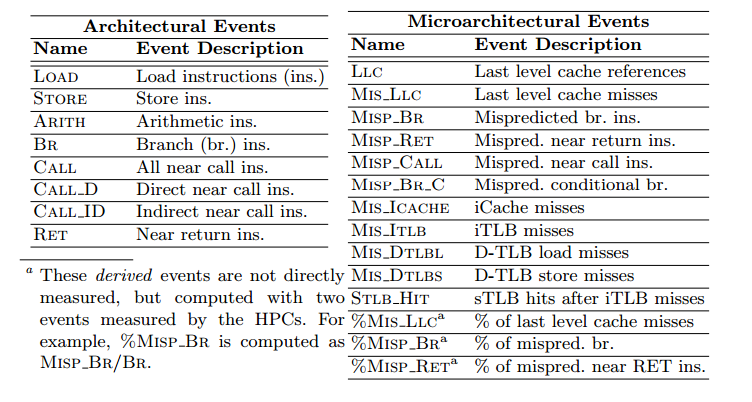
\includegraphics[width=4in]{img/tracking_events.png}
	\caption{shortlisted candidate events to be monitored}
\end{figure}


\bibliography{week1}{}
\bibliographystyle{plain}
\end{document}

